% Options for packages loaded elsewhere
\PassOptionsToPackage{unicode}{hyperref}
\PassOptionsToPackage{hyphens}{url}
\PassOptionsToPackage{dvipsnames,svgnames,x11names}{xcolor}
%
\documentclass[
]{article}

\usepackage{amsmath,amssymb}
\usepackage{iftex}
\ifPDFTeX
  \usepackage[T1]{fontenc}
  \usepackage[utf8]{inputenc}
  \usepackage{textcomp} % provide euro and other symbols
\else % if luatex or xetex
  \usepackage{unicode-math}
  \defaultfontfeatures{Scale=MatchLowercase}
  \defaultfontfeatures[\rmfamily]{Ligatures=TeX,Scale=1}
\fi
\usepackage{lmodern}
\ifPDFTeX\else  
    % xetex/luatex font selection
\fi
% Use upquote if available, for straight quotes in verbatim environments
\IfFileExists{upquote.sty}{\usepackage{upquote}}{}
\IfFileExists{microtype.sty}{% use microtype if available
  \usepackage[]{microtype}
  \UseMicrotypeSet[protrusion]{basicmath} % disable protrusion for tt fonts
}{}
\makeatletter
\@ifundefined{KOMAClassName}{% if non-KOMA class
  \IfFileExists{parskip.sty}{%
    \usepackage{parskip}
  }{% else
    \setlength{\parindent}{0pt}
    \setlength{\parskip}{6pt plus 2pt minus 1pt}}
}{% if KOMA class
  \KOMAoptions{parskip=half}}
\makeatother
\usepackage{xcolor}
\usepackage[lmargin=1.25in,rmargin=1.25in,tmargin=1in,bmargin=1in]{geometry}
\setlength{\emergencystretch}{3em} % prevent overfull lines
\setcounter{secnumdepth}{5}
% Make \paragraph and \subparagraph free-standing
\makeatletter
\ifx\paragraph\undefined\else
  \let\oldparagraph\paragraph
  \renewcommand{\paragraph}{
    \@ifstar
      \xxxParagraphStar
      \xxxParagraphNoStar
  }
  \newcommand{\xxxParagraphStar}[1]{\oldparagraph*{#1}\mbox{}}
  \newcommand{\xxxParagraphNoStar}[1]{\oldparagraph{#1}\mbox{}}
\fi
\ifx\subparagraph\undefined\else
  \let\oldsubparagraph\subparagraph
  \renewcommand{\subparagraph}{
    \@ifstar
      \xxxSubParagraphStar
      \xxxSubParagraphNoStar
  }
  \newcommand{\xxxSubParagraphStar}[1]{\oldsubparagraph*{#1}\mbox{}}
  \newcommand{\xxxSubParagraphNoStar}[1]{\oldsubparagraph{#1}\mbox{}}
\fi
\makeatother

\usepackage{color}
\usepackage{fancyvrb}
\newcommand{\VerbBar}{|}
\newcommand{\VERB}{\Verb[commandchars=\\\{\}]}
\DefineVerbatimEnvironment{Highlighting}{Verbatim}{commandchars=\\\{\}}
% Add ',fontsize=\small' for more characters per line
\usepackage{framed}
\definecolor{shadecolor}{RGB}{241,243,245}
\newenvironment{Shaded}{\begin{snugshade}}{\end{snugshade}}
\newcommand{\AlertTok}[1]{\textcolor[rgb]{0.68,0.00,0.00}{#1}}
\newcommand{\AnnotationTok}[1]{\textcolor[rgb]{0.37,0.37,0.37}{#1}}
\newcommand{\AttributeTok}[1]{\textcolor[rgb]{0.40,0.45,0.13}{#1}}
\newcommand{\BaseNTok}[1]{\textcolor[rgb]{0.68,0.00,0.00}{#1}}
\newcommand{\BuiltInTok}[1]{\textcolor[rgb]{0.00,0.23,0.31}{#1}}
\newcommand{\CharTok}[1]{\textcolor[rgb]{0.13,0.47,0.30}{#1}}
\newcommand{\CommentTok}[1]{\textcolor[rgb]{0.37,0.37,0.37}{#1}}
\newcommand{\CommentVarTok}[1]{\textcolor[rgb]{0.37,0.37,0.37}{\textit{#1}}}
\newcommand{\ConstantTok}[1]{\textcolor[rgb]{0.56,0.35,0.01}{#1}}
\newcommand{\ControlFlowTok}[1]{\textcolor[rgb]{0.00,0.23,0.31}{\textbf{#1}}}
\newcommand{\DataTypeTok}[1]{\textcolor[rgb]{0.68,0.00,0.00}{#1}}
\newcommand{\DecValTok}[1]{\textcolor[rgb]{0.68,0.00,0.00}{#1}}
\newcommand{\DocumentationTok}[1]{\textcolor[rgb]{0.37,0.37,0.37}{\textit{#1}}}
\newcommand{\ErrorTok}[1]{\textcolor[rgb]{0.68,0.00,0.00}{#1}}
\newcommand{\ExtensionTok}[1]{\textcolor[rgb]{0.00,0.23,0.31}{#1}}
\newcommand{\FloatTok}[1]{\textcolor[rgb]{0.68,0.00,0.00}{#1}}
\newcommand{\FunctionTok}[1]{\textcolor[rgb]{0.28,0.35,0.67}{#1}}
\newcommand{\ImportTok}[1]{\textcolor[rgb]{0.00,0.46,0.62}{#1}}
\newcommand{\InformationTok}[1]{\textcolor[rgb]{0.37,0.37,0.37}{#1}}
\newcommand{\KeywordTok}[1]{\textcolor[rgb]{0.00,0.23,0.31}{\textbf{#1}}}
\newcommand{\NormalTok}[1]{\textcolor[rgb]{0.00,0.23,0.31}{#1}}
\newcommand{\OperatorTok}[1]{\textcolor[rgb]{0.37,0.37,0.37}{#1}}
\newcommand{\OtherTok}[1]{\textcolor[rgb]{0.00,0.23,0.31}{#1}}
\newcommand{\PreprocessorTok}[1]{\textcolor[rgb]{0.68,0.00,0.00}{#1}}
\newcommand{\RegionMarkerTok}[1]{\textcolor[rgb]{0.00,0.23,0.31}{#1}}
\newcommand{\SpecialCharTok}[1]{\textcolor[rgb]{0.37,0.37,0.37}{#1}}
\newcommand{\SpecialStringTok}[1]{\textcolor[rgb]{0.13,0.47,0.30}{#1}}
\newcommand{\StringTok}[1]{\textcolor[rgb]{0.13,0.47,0.30}{#1}}
\newcommand{\VariableTok}[1]{\textcolor[rgb]{0.07,0.07,0.07}{#1}}
\newcommand{\VerbatimStringTok}[1]{\textcolor[rgb]{0.13,0.47,0.30}{#1}}
\newcommand{\WarningTok}[1]{\textcolor[rgb]{0.37,0.37,0.37}{\textit{#1}}}

\providecommand{\tightlist}{%
  \setlength{\itemsep}{0pt}\setlength{\parskip}{0pt}}\usepackage{longtable,booktabs,array}
\usepackage{calc} % for calculating minipage widths
% Correct order of tables after \paragraph or \subparagraph
\usepackage{etoolbox}
\makeatletter
\patchcmd\longtable{\par}{\if@noskipsec\mbox{}\fi\par}{}{}
\makeatother
% Allow footnotes in longtable head/foot
\IfFileExists{footnotehyper.sty}{\usepackage{footnotehyper}}{\usepackage{footnote}}
\makesavenoteenv{longtable}
\usepackage{graphicx}
\makeatletter
\newsavebox\pandoc@box
\newcommand*\pandocbounded[1]{% scales image to fit in text height/width
  \sbox\pandoc@box{#1}%
  \Gscale@div\@tempa{\textheight}{\dimexpr\ht\pandoc@box+\dp\pandoc@box\relax}%
  \Gscale@div\@tempb{\linewidth}{\wd\pandoc@box}%
  \ifdim\@tempb\p@<\@tempa\p@\let\@tempa\@tempb\fi% select the smaller of both
  \ifdim\@tempa\p@<\p@\scalebox{\@tempa}{\usebox\pandoc@box}%
  \else\usebox{\pandoc@box}%
  \fi%
}
% Set default figure placement to htbp
\def\fps@figure{htbp}
\makeatother

\pagenumbering{gobble}
\usepackage{scrlayer-scrpage}
\rohead{Batch Processing Tutorial V2.0}
\usepackage[noblocks]{authblk}
\renewcommand*{\Authsep}{, }
\renewcommand*{\Authand}{ and }
\renewcommand*{\Authands}{, }
\renewcommand\Affilfont{\small}
\makeatletter
\@ifpackageloaded{tcolorbox}{}{\usepackage[skins,breakable]{tcolorbox}}
\@ifpackageloaded{fontawesome5}{}{\usepackage{fontawesome5}}
\definecolor{quarto-callout-color}{HTML}{909090}
\definecolor{quarto-callout-note-color}{HTML}{0758E5}
\definecolor{quarto-callout-important-color}{HTML}{CC1914}
\definecolor{quarto-callout-warning-color}{HTML}{EB9113}
\definecolor{quarto-callout-tip-color}{HTML}{00A047}
\definecolor{quarto-callout-caution-color}{HTML}{FC5300}
\definecolor{quarto-callout-color-frame}{HTML}{acacac}
\definecolor{quarto-callout-note-color-frame}{HTML}{4582ec}
\definecolor{quarto-callout-important-color-frame}{HTML}{d9534f}
\definecolor{quarto-callout-warning-color-frame}{HTML}{f0ad4e}
\definecolor{quarto-callout-tip-color-frame}{HTML}{02b875}
\definecolor{quarto-callout-caution-color-frame}{HTML}{fd7e14}
\makeatother
\makeatletter
\@ifpackageloaded{caption}{}{\usepackage{caption}}
\AtBeginDocument{%
\ifdefined\contentsname
  \renewcommand*\contentsname{Table of contents}
\else
  \newcommand\contentsname{Table of contents}
\fi
\ifdefined\listfigurename
  \renewcommand*\listfigurename{List of Figures}
\else
  \newcommand\listfigurename{List of Figures}
\fi
\ifdefined\listtablename
  \renewcommand*\listtablename{List of Tables}
\else
  \newcommand\listtablename{List of Tables}
\fi
\ifdefined\figurename
  \renewcommand*\figurename{Figure}
\else
  \newcommand\figurename{Figure}
\fi
\ifdefined\tablename
  \renewcommand*\tablename{Table}
\else
  \newcommand\tablename{Table}
\fi
}
\@ifpackageloaded{float}{}{\usepackage{float}}
\floatstyle{ruled}
\@ifundefined{c@chapter}{\newfloat{codelisting}{h}{lop}}{\newfloat{codelisting}{h}{lop}[chapter]}
\floatname{codelisting}{Listing}
\newcommand*\listoflistings{\listof{codelisting}{List of Listings}}
\makeatother
\makeatletter
\makeatother
\makeatletter
\@ifpackageloaded{caption}{}{\usepackage{caption}}
\@ifpackageloaded{subcaption}{}{\usepackage{subcaption}}
\makeatother

\usepackage{bookmark}

\IfFileExists{xurl.sty}{\usepackage{xurl}}{} % add URL line breaks if available
\urlstyle{same} % disable monospaced font for URLs
\hypersetup{
  pdftitle={Batch Processing in PAMGuard},
  pdfauthor={Douglas Gillespie},
  colorlinks=true,
  linkcolor={blue},
  filecolor={Maroon},
  citecolor={Blue},
  urlcolor={Blue},
  pdfcreator={LaTeX via pandoc}}


\title{Batch Processing in PAMGuard}


\author[1]{Douglas Gillespie}

\affil[1]{Sea Mammal Research Unit, University of St Andrews}


\date{2025-03-20}
\begin{document}
\maketitle

\centerline{\textbf{Tutorial Version 2.0}}
\vspace{3cm}


\centerline{\textbf{Learning Outcomes}}

In this tutorial you wil learn to:
\begin{enumerate}
\item Learn what we mean by batch processing
\item Install the Batch Processor in PAMGurd
\item Set up a PAMGuard configuration to run batch processes
\item Run a process of a multiple sets of raw data files
\item Run additional offline tasks on the generated PAMGuard output
\end{enumerate}
\newpage

\renewcommand*\contentsname{Table of contents}
{
\hypersetup{linkcolor=}
\setcounter{tocdepth}{3}
\tableofcontents
}
\listoffigures

\newpage{}

\pagenumbering{arabic}
\pagestyle{plain}

\section{Introduction}\label{introduction}

The Batch processor currently only works on Windows computers. We hope
to bring out a Mac version later in 2025.

Help pages for the batch processor are available from the PAMGuard Help
menu, or
\href{https://www.pamguard.org/batchhelp/docs/batchoverview.html}{here
online}.

The PAMGuard batch processing module allows you to run the same PAMGuard
configuration on multiple sets of data (Figure~\ref{fig-normaldiagram}).
This is particularly useful if you want to process data from deployments
of multiple autonomous recorders in exactly the same way. It can also be
used to reprocess data from multiple old cruises with a new detector,
for instance with one of the new Deep Learning detectors / classifiers
that have recently been added to PAMGuard.

\begin{tcolorbox}[enhanced jigsaw, titlerule=0mm, bottomrule=.15mm, leftrule=.75mm, coltitle=black, breakable, colframe=quarto-callout-tip-color-frame, left=2mm, toptitle=1mm, rightrule=.15mm, colback=white, bottomtitle=1mm, colbacktitle=quarto-callout-tip-color!10!white, opacityback=0, title=\textcolor{quarto-callout-tip-color}{\faLightbulb}\hspace{0.5em}{PAMGuard configuration files}, arc=.35mm, opacitybacktitle=0.6, toprule=.15mm]

PAMGuard configurations are held in psfx files. They contain all of the
information about the modules you've selected and how you've configured
those modules.

They can be easily copied or emailed between users.

\end{tcolorbox}

PAMGuard users will know that setting up the same configurations on
multiple datasets is tiresome. For each dataset, you need to copy the
configuration (psfx) file, then change the input folder for your sound
files, the output folder for the binary data and the output database. If
you get this wrong, then you might overwrite some data. Then, when you
decide that those weren't exactly the detector settings you wanted, you
have to do it all again for all your data sets.

The PAMGuard batch processing module addresses this problem by running
the same configuration on as many data sets as you want. You set up a
series of ``jobs'', and the batch processor will work through them,
using the same configuration, until they are complete. Generally, it
will run multiple jobs concurrently on a single machine.

As well as processing raw audio data, it can also run `offline tasks' on
already processed data. For instance if you wanted to change the click
classifier settings, and reprocess all of the click binary files in
multiple datasets, the batch processor can help do this in an efficient
manner.

\begin{tcolorbox}[enhanced jigsaw, titlerule=0mm, bottomrule=.15mm, leftrule=.75mm, coltitle=black, breakable, colframe=quarto-callout-note-color-frame, left=2mm, toptitle=1mm, rightrule=.15mm, colback=white, bottomtitle=1mm, colbacktitle=quarto-callout-note-color!10!white, opacityback=0, title=\textcolor{quarto-callout-note-color}{\faInfo}\hspace{0.5em}{My personal data processing record}, arc=.35mm, opacitybacktitle=0.6, toprule=.15mm]

My personal record is reprocessing over 80 Terrabytes of multibeam
active sonar data, spread over 14 external USB hard drives, in less than
8 days. Do achieve this, I set up 6 jobs processing data on the first 6
hard drives, with the desktop PC set to run three jobs at a time. When
the first three jobs were complete I replaced those hard drives and set
up the next three jobs, and so on until processing was complete. In all,
it only required half an hour or so of my time every 2 or 3 days.

Data from this analysis are in the recent paper
\href{https://doi.org/10.1111/1365-2664.14844}{Montabaranom et al.~Seals
exhibit localised avoidance of operational tidal turbines}.

\end{tcolorbox}

\begin{figure}

\centering{

\pandocbounded{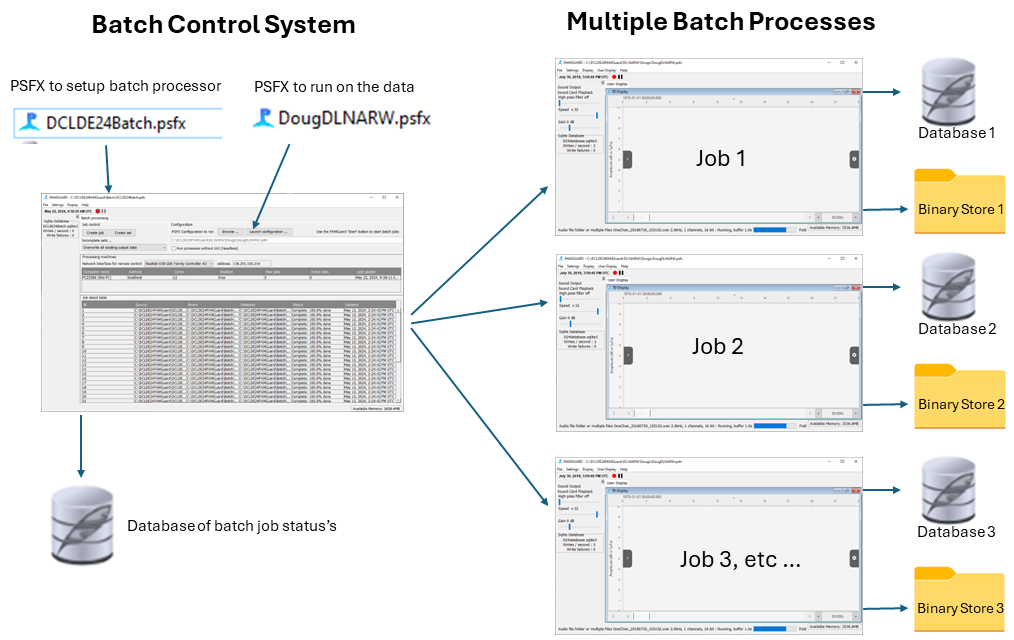
\includegraphics[keepaspectratio]{images/normaldiagram.png}}

}

\caption{\label{fig-normaldiagram}Diagram of the batch processor
configuration}

\end{figure}%

\subsection{Soundtraps}\label{soundtraps}

SoundTraps are slightly more sophisticated than many recorders.
Depending on how they are configured, they may not just be recording raw
audio data, but also the output of an onboard detector. The ones we're
using were configured to sample raw data at a sample rate of 576kHz. The
soundtrap then ran an automatic transient (click) detector on the
incoming data and each detection was saved as a short clip just over a
millisecond long. The incoming high frequency data were then decimated
to 96kHz and all of the 96kHz data stored. Both the detections and the
recordings are compressed using a lossless compression algorithm and
stored together in a SUD file as shown in
Figure~\ref{fig-soundtrapflow}.

\begin{figure}

\centering{

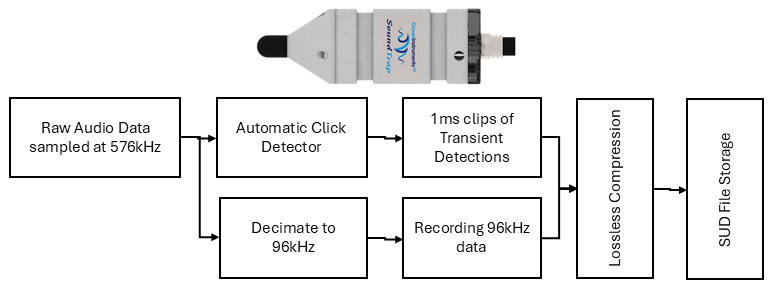
\includegraphics[width=0.9\linewidth,height=\textheight,keepaspectratio]{images/soundtrapflow.png}

}

\caption{\label{fig-soundtrapflow}Schematic diagram of the data flow
through a soundtrap}

\end{figure}%

The soundtrap system does not attempt to run automatic detectors for
lower frequency sounds. This would be too complicated for the low power
processor that soundtraps use. The combination of high frequency click
detection and lower frequency recording allows us to detect the very
high frequency clicks of species such as the harbour porpoise, and at
the same time, make recordings which can be processed offline for a wide
variety of other species. This system allows for much longer deployments
than would be possible if all of the high frequency data were recorded.
For more information about soundtraps, visit the
\href{https://www.oceaninstruments.co.nz/}{Ocean Instruments} web pages.

This tutorial follows on directly from another PAMGuard Tutorial
\href{https://www.pamguard.org/tutorials/staticmonitoring.html}{Introduction
to Static Monitoring} which you might want to complete before proceeding
with this tutorial, which will focus on batch processing with a
pre-built configuration.

\section{Installation}\label{installation}

\subsection{Software}\label{software}

This tutorial will work with PAMGuard Version 2.02.16 or later and the
Batch Processor Plugin version 2.0 or later, both of which are available
on the PAMGuard website. Once you've installed PAMGuard, copy the
downloaded Batch module (BatchProcessing\_2\_0.jar) into the plugins
folder, which you'll find in your PAMGuard installation folder (probably
C:\textbackslash Program
Files\textbackslash Pamguard\textbackslash plugins). If you've any older
versions of the Batch Processor plugin in that folder, make sure you
remove them. Once this is done, the Batch Processor module will appear
in the Add Modules / Utilities menu just like any other PAMGuard module,
and it's help pages will be available in the PAMGuard online help.

\subsection{Sample Data}\label{sample-data}

The data you'll be using for this tutorial come from a deployment of
five SoundTrap 300 recorders off the West coast of Scotland, which form
part of the
\href{https://www.sams.ac.uk/science/projects/compass/}{Compass
Project}. We've taken a single days data for each recorder since the
full dataset would be too large for a tutorial exercise and might take
many days to process.

The data are available on Zenodo at
\url{https://zenodo.org/uploads/14989668}. The Zenodo dataset contains
the following files:

\begin{Shaded}
\begin{Highlighting}[]
\NormalTok{├── soundtrapdata.zip                  \#Five example days of acoustic recordings}
\NormalTok{│   ├── Hyskier                        \#Folder of files for the Hyskier site}
\NormalTok{│   ├── ShiantIsles                    \# etc.}
\NormalTok{│   ├── StantonBank}
\NormalTok{│   ├── StoerHead}
\NormalTok{│   ├── Tolsta}
\NormalTok{├── README.md                          \#This readme file}
\NormalTok{├── CompassMetaData.csv                \#Calibration and location data for each device}
\NormalTok{├── compass\_settings\_static\_logger.psfx \#PAMGuard configuration for data processing}
\NormalTok{└── PAMGuardOutput.zip                 \#Processed data from the five deployments}
\NormalTok{│   ├── Hyskier\_binary                 \#Folder of binary file output for the Hyskier site}
\NormalTok{│   ├── ShiantIsles\_binary             \# etc.}
\NormalTok{│   ├── StantonBank\_binary }
\NormalTok{│   ├── StoerHead\_binary }
\NormalTok{│   ├── Tolsta\_binary }
\NormalTok{│   ├── Hyskier\_database.sqlite3       \# SQLite database output for the Hyskier site}
\NormalTok{│   ├── ShiantIsles\_database.sqlite3   \# etc.}
\NormalTok{│   ├── StantonBank\_database.sqlite3 }
\NormalTok{│   ├── StoerHead\_database.sqlite3 }
\NormalTok{│   └── Tolsta\_database.sqlite3 }
\end{Highlighting}
\end{Shaded}

For this tutorial you only need soundtrapdata.zip,
compass\_settings\_static\_logger.psfx, and CompassMetaData.csv. You'll
be recreating the files in PAMGuardOutput.zip, so you don't need them,
but take a look if you want to.

Unzip soundtrapdata.zip and copy the other files to a convenient
location on your hard drive.

\section{Configure PAMGuard}\label{configure-pamguard}

Two PAMGuard configurations are required to run the batch processor. A
configuration that contains the PAMGuard modules that you want to run on
your data, and a second configuration that is going to control the Batch
Processor. We'll call these the \textbf{Run configuration} and the
\textbf{Batch Configuration} respectively.

\subsection{The Run configuration}\label{the-run-configuration}

The run configuration you'll be using is the configuration you should
have ended up with at the end of the
\href{https://www.pamguard.org/tutorials/staticmonitoring.html}{Introduction
to Static Monitoring} tutorial. If you completed the static monitoring
tutorial, you can use the configuration you had at the end, or you can
use compass\_settings\_static\_logger.psfx which you should have
downloaded in configuration.zip for this tutorial.

The configuration (Figure~\ref{fig-pamguardmodel}) uses an FFT module to
compute a spectrogram of the 96kHz data which feeds a Whistle detector
and a long team spectral average (LTSA) generator. The 96kHz data also
input to a Noise band Monitor and are also decimated to 10kHz fo feed a
second copy of the Whislte and Moan detector to search for lower
frequency tonal sounds. You'll also see the ``ST Click Detector'' which
is not connected to the data from the sound acquisition. This is because
it's a special version of the click detector, modified to receive the
detection clips from the SUD files, which you'll remember are at the
higher sample rate of 576kHz.

\begin{figure}

\centering{

\pandocbounded{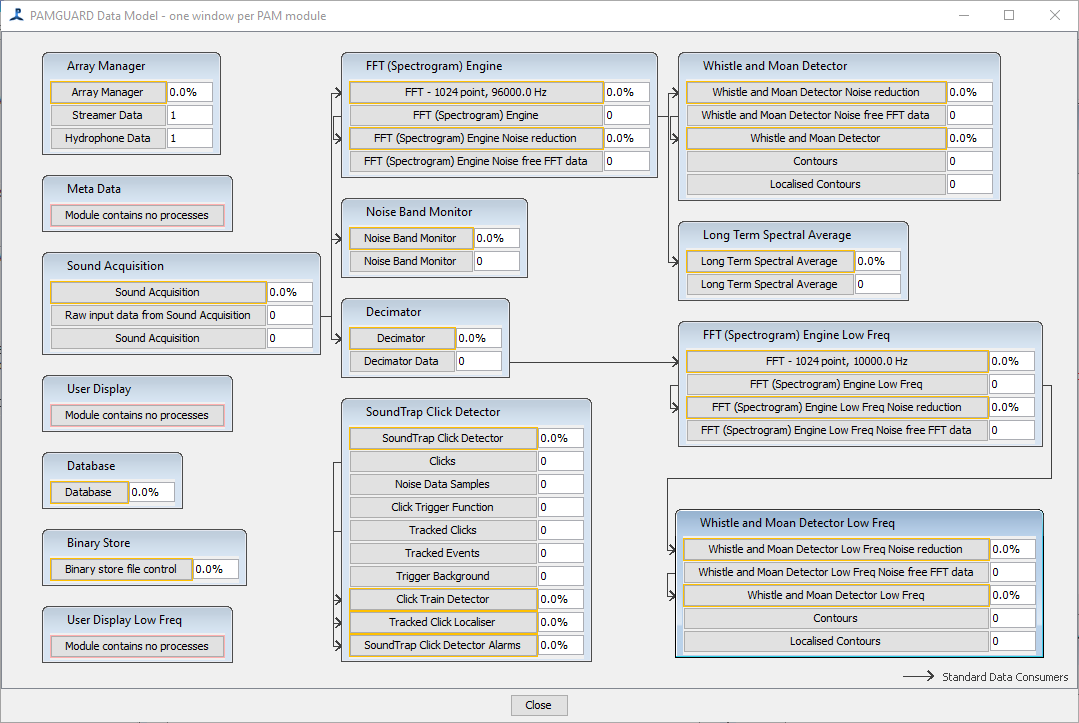
\includegraphics[keepaspectratio]{images/pamguardmodel.png}}

}

\caption{\label{fig-pamguardmodel}PAMGuard Data Model Diagram for
SoundTrapClicksNWsls.psfx}

\end{figure}%

As well as the above sound processing and detection modules, there is
the Array Manager and Meta Data modules (both always present in every
PAMGuard configuration), a Binary Store and Database for the output data
we're about to generate, and a User Display which will show a
spectrogram of the 96kHz data overlaid with whistle detections.

You've probably opened the compass\_settings\_static\_logger.psfx file
yourself by now. Close it again before you start to create the Batch
Configuration.

\subsection{The Batch Configuration}\label{the-batch-configuration}

You'll be making the batch configuration from scratch so that you learn
to use the batch processor.

Start PAMGuard and create a new configuration: launch PAMGuard from the
Windows Start menu, and when it asks you to ``load PAMGuard
configuration from \ldots{}'' press \textbf{Browse / Create New\ldots{}}
. In the dialog that opens, navigate to where you want to work, and
enter the file name CompassBatch (Figure~\ref{fig-createpsfx}), then hit
the Select button or press Enter.

\begin{figure}

\centering{

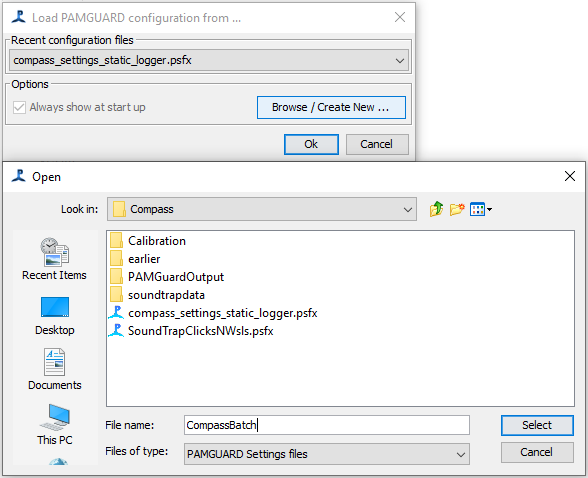
\includegraphics[width=0.7\linewidth,height=\textheight,keepaspectratio]{images/createpsfx.png}

}

\caption{\label{fig-createpsfx}PAMGuard dialog for creating a new
configuration file}

\end{figure}%

From PAMGuards \emph{File / add modules / utilities} menu add a Database
and a Batch processing module to the configuration. Then from the
\emph{File / Database / Database Selection} menu dialog, press
\textbf{Browse / Create \ldots{}}, and enter the name of the database
(e.g.~CompassBatch) which is going to hold information about the jobs
you're running and how they are progressing. Your PAMGuard configuration
should now look like Figure~\ref{fig-emptyconfig} .

\begin{figure}

\centering{

\pandocbounded{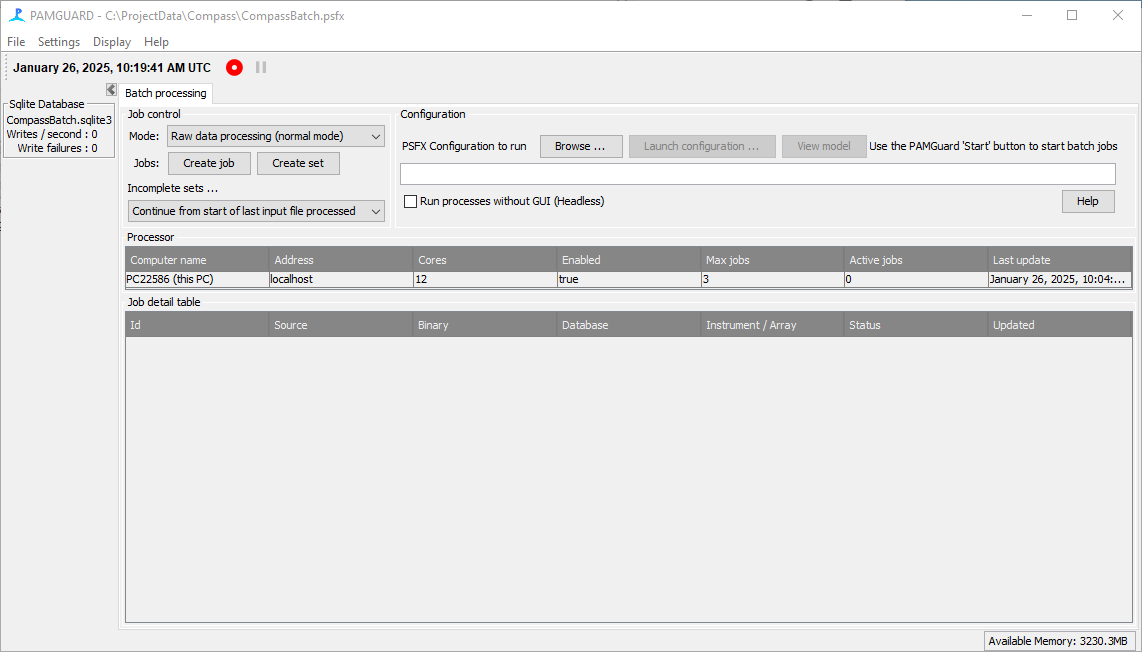
\includegraphics[keepaspectratio]{images/emptyconfig.png}}

}

\caption{\label{fig-emptyconfig}PAMGuard configuration with database and
batch processor modules}

\end{figure}%

\subsubsection{Select the configuration
file}\label{select-the-configuration-file}

At the top of the display, in the configuration panel, press the
\textbf{Browse \ldots{}} button and select the Run Configuration
compass\_settings\_static\_logger.psfx.

\subsection{Create jobs}\label{create-jobs}

You should have five sets of sud files, downloaded from
\href{https://zenodo.org/uploads/14989668}{Zenodo}, each in a different
folder. You can create all five jobs at once from the \textbf{Create
Set} button in the Job Control Panel. Press the \textbf{Create Set}
button, then in the dialog, press the \textbf{Select button} in the top
right corner. Navigate to the folder containing the five folders of
soundtrap data and select just that root folder (in the example in
Figure~\ref{fig-createset} it's
C:\textbackslash ProjectData\textbackslash Compass\textbackslash soundtrapdata).

\begin{figure}

\centering{

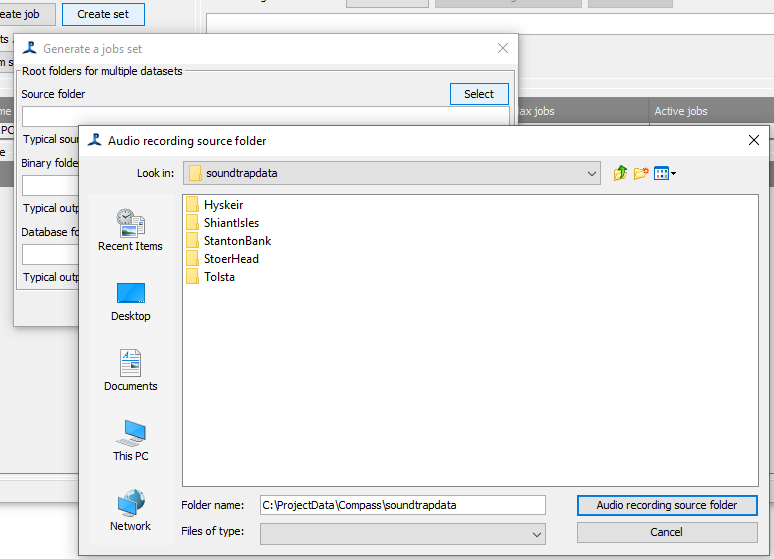
\includegraphics[width=0.7\linewidth,height=\textheight,keepaspectratio]{images/createset.png}

}

\caption{\label{fig-createset}Selecting the source folder for multiple
batch jobs}

\end{figure}%

The Batch processor will only look one level of folders down from the
folder you select, so make sure you've selected the right folder. If
you've got it right, you'll be told that its found five sub folders
containing data.

Next select folders for the binary output and for the databases that
will be automatically generated. I've chosen the folder
C:\textbackslash ProjectData\textbackslash Compass\textbackslash PAMGuardOutput
for both.

Press OK, and the set of five batch jobs should show in the main
PAMGuard batch display (Figure~\ref{fig-config2}). If you look at your
folders and files with Windows Explorer, you'll not see any of the
output binary folders and databases at this stage. Don't worry, they
will be created automatically as each batch job starts.

\begin{figure}

\centering{

\pandocbounded{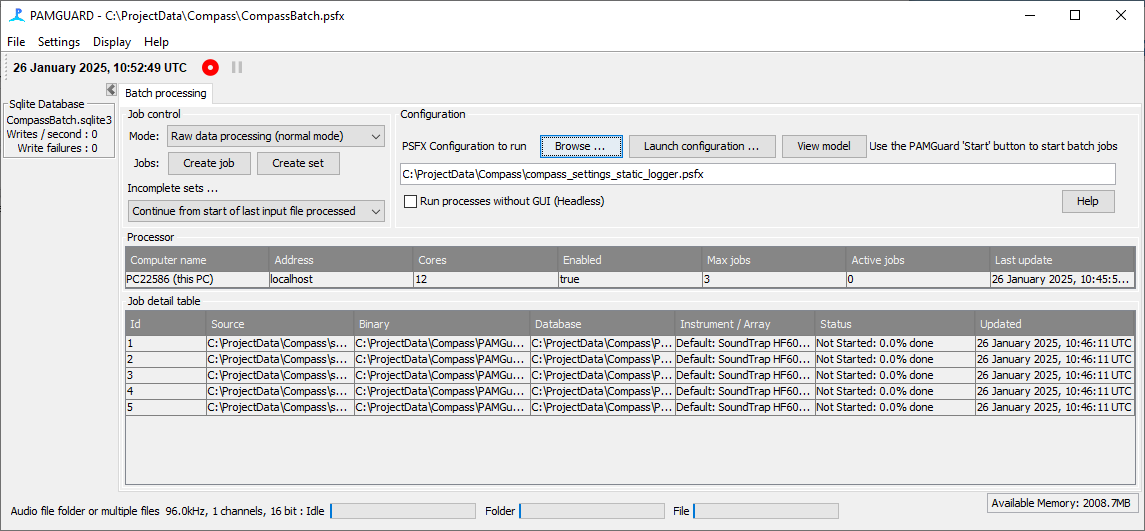
\includegraphics[keepaspectratio]{images/config2.png}}

}

\caption{\label{fig-config2}PAMGuard configuration with a set of five
batch jobs}

\end{figure}%

\subsection{Set individual job calibration and location
data.}\label{set-individual-job-calibration-and-location-data.}

By default, the batch processor will take hydrophone data from the Run
Configuration and use it with each set of data processes. If you're
making noise measurements, you will need to set the correct hydrophone
calibration values for each job, or the noise measurements will not be
accurate. If you're processing data from static hydrophones, you may
also want to set the correct location of each deployment.

Calibration and location values for each dataset are provided in the
file CompassMetaData.csv.

\begin{figure}

\begin{minipage}{\linewidth}

\centering{

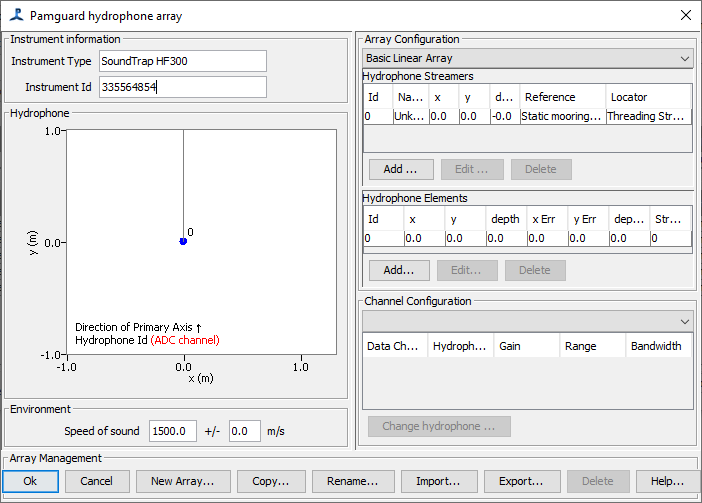
\includegraphics[width=0.7\linewidth,height=\textheight,keepaspectratio]{images/arraymanager1.png}

}

\subcaption{\label{fig-arraymanager1}Array Manager dialog panel}

\end{minipage}%
\newline
\begin{minipage}{0.38\linewidth}

\centering{

\pandocbounded{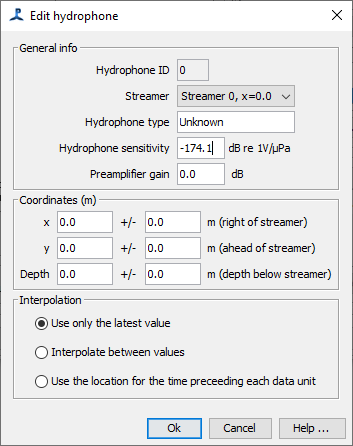
\includegraphics[keepaspectratio]{images/hydrophone.png}}

}

\subcaption{\label{fig-hydrophone}Hydrophone Sensitivity}

\end{minipage}%
%
\begin{minipage}{0.02\linewidth}
~\end{minipage}%
%
\begin{minipage}{0.60\linewidth}

\centering{

\pandocbounded{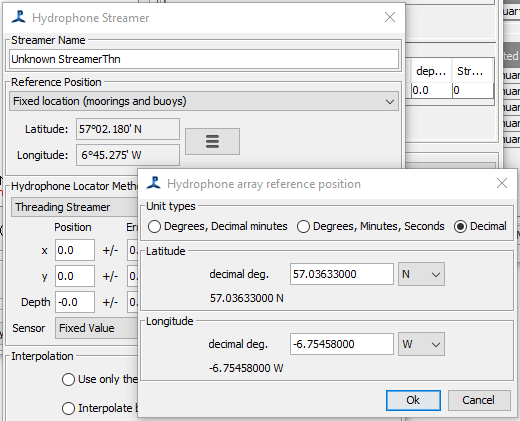
\includegraphics[keepaspectratio]{images/array.png}}

}

\subcaption{\label{fig-array}Location Data}

\end{minipage}%

\caption{\label{fig-arrayman}Entering the hydrophone calibration and
location data}

\end{figure}%

For each job in the table, right click on the row and select \emph{Add
or Edit calibration / Array Data} from the dropdown menu. This will open
the Array Manager dialog (Figure~\ref{fig-arraymanager1}), using the
current default values from the Run Configuration. Enter the SoundTrap
serial number in the Instrument Id field. Next double click on the
hydrophone element (there is only one for this SoundTrap). Enter the
hydrophone sensitivity as the negative of the High Gain full scale value
from the spreadsheet (Figure~\ref{fig-hydrophone}). Then open the
`streamer', again by double clicking or by pressing the \emph{Edit}
button. Right click on the menu button to the right of the display
position and select \emph{Edit} from the dropdown menu. When the
Hydrophone array reference position dialog opens, click on ``Decimal''
in the top right hand corner and copy/paste the appropriate values from
the spreadsheet (Figure~\ref{fig-array}).

Work your way through all five jobs and set the data for all of them.

\begin{tcolorbox}[enhanced jigsaw, titlerule=0mm, bottomrule=.15mm, leftrule=.75mm, coltitle=black, breakable, colframe=quarto-callout-important-color-frame, left=2mm, toptitle=1mm, rightrule=.15mm, colback=white, bottomtitle=1mm, colbacktitle=quarto-callout-important-color!10!white, opacityback=0, title=\textcolor{quarto-callout-important-color}{\faExclamation}\hspace{0.5em}{Feedback}, arc=.35mm, opacitybacktitle=0.6, toprule=.15mm]

We agree that this can be a bit of a pain for a deployment of many
recorders and are trying to think of an easier way of doing this, such
as importing data from a database or spreadsheet.

\end{tcolorbox}

\section{Run the batch jobs}\label{run-the-batch-jobs}

\subsection{Number of concurrent jobs}\label{number-of-concurrent-jobs}

The final thing to decide before starting processing is how many
concurrent jobs your computer can manage efficiently. How many jobs can
run concurrently depends on the complexity of the configuration and on
how powerful the computer is. On a good Intel I7 desktop with 32 GBytes
of RAM and 20 processor cores, I'd probably run three jobs at a time. On
my laptop, which only has 12 cores and 16 GByte RAM, I'll stick to 2. To
set the number of jobs right click on the Processor table (which will
have a single line in it for your current machine) and either increase
or decrease the maximum number of jobs.

\subsection{Run the jobs}\label{run-the-jobs}

\begin{figure}

\centering{

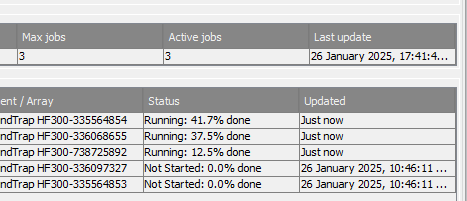
\includegraphics[width=0.5\linewidth,height=\textheight,keepaspectratio]{images/jobstatus.png}

}

\caption{\label{fig-jobstatus}Batch Job Status}

\end{figure}%

You're now ready to start the batch jobs. Press the PAMGuard start
button and wait a few seconds for the first jobs to start. The jobs
table will show the status of each job (Figure~\ref{fig-jobstatus}),
which will update as each processed file completes. When a job ends,
another will start until all jobs are complete.

Look in the folder where you've told it to put the binary files and
databases. You should see database files and folders of binary output
start to appear as each job runs.

You can change the number of concurrent jobs while they are running. If
you reduce the number, then no jobs will be stopped, but when one ends,
another will not start until the number of active jobs drops below the
set maximum. If you increase the number of jobs, another job will start
immediately.

Once jobs are complete, there will be a menu option available to open
that dataset with the PAMGuard Viewer. For further information, see the
online help.

\begin{tcolorbox}[enhanced jigsaw, titlerule=0mm, bottomrule=.15mm, leftrule=.75mm, coltitle=black, breakable, colframe=quarto-callout-tip-color-frame, left=2mm, toptitle=1mm, rightrule=.15mm, colback=white, bottomtitle=1mm, colbacktitle=quarto-callout-tip-color!10!white, opacityback=0, title=\textcolor{quarto-callout-tip-color}{\faLightbulb}\hspace{0.5em}{Impatient ?}, arc=.35mm, opacitybacktitle=0.6, toprule=.15mm]

Unless you have a powerful computer, running these sample jobs may take
an hour or more. At this point you may want to stop the jobs and take a
look at the preprocessed data we provided for you.

\end{tcolorbox}

\section{Running Offline Tasks}\label{running-offline-tasks}

Several PAMGuard modules have options in Viewer mode to re-run certain
tasks, such as click classification.

Indeed, in the exercises above, we deliberately `forgot' to set up the
SoundTrap click detector to classify porpoise clicks, so we should run
that task now.

To run offline tasks go back to your batch configuration then in the top
of the Job Control Panel, select Mode: Offline tasks (viewer mode) from
the two options. (You could also start an entirely new batch
configuration, and set up the jobs again, but that's not necessary for
us here). The display will change to also show a table of possible
offline tasks to run on the data (Figure~\ref{fig-offconfig}). Note that
you may have to resize the display and move the dividers between the
different tables to see this properly. Also, if you're now using the
pre-processed data, the paths to the data in your batch configuration
might all be wrong, so check them!

\subsection{Configure a click reclassification
task}\label{configure-a-click-reclassification-task}

\begin{figure}

\centering{

\pandocbounded{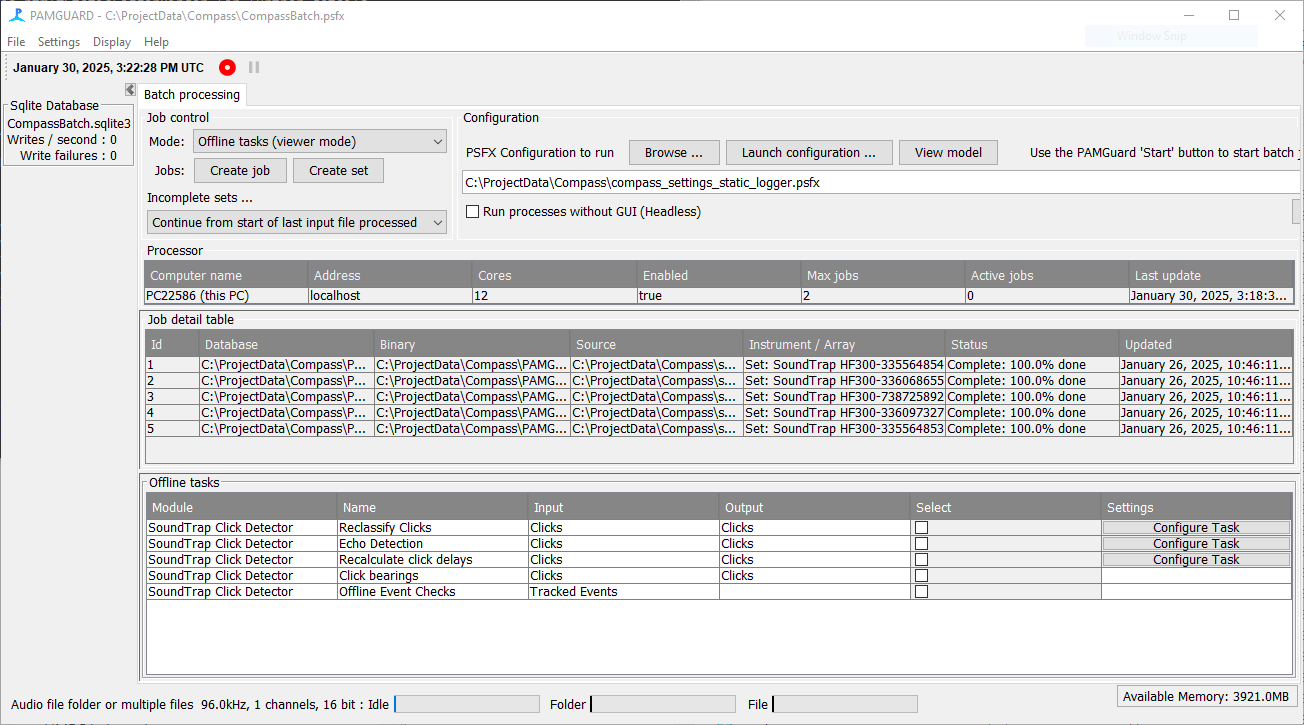
\includegraphics[keepaspectratio]{images/offlineconfig.png}}

}

\caption{\label{fig-offconfig}Configuration display for controlling
offline tasks}

\end{figure}%

The batch processor will have automatically extracted a list of
available tasks from the modules in your run configuration. In this
case, there are five tasks, all from the click detector. Recalculating
delays and bearings is not relevant to single channel data, but we can
run the click classification. Click on the \textbf{Configure Task}
button for Reclassify Clicks, then in the dialog
(Figure~\ref{fig-reclass1}), then press the \textbf{New} button to open
the Click Parameters dialog (Figure~\ref{fig-reclass2}). In the bottom
right from \textbf{Set Defaults} select \emph{Porpoise} which will set
default values for porpoise click classification.

\begin{figure}

\begin{minipage}{0.45\linewidth}

\centering{

\pandocbounded{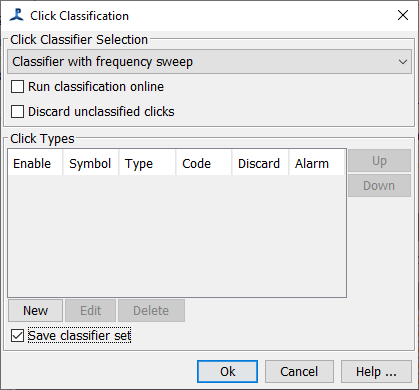
\includegraphics[keepaspectratio]{images/reclass1.png}}

}

\subcaption{\label{fig-reclass1}Click Reclassification configuration}

\end{minipage}%
%
\begin{minipage}{0.01\linewidth}
~\end{minipage}%
%
\begin{minipage}{0.55\linewidth}

\centering{

\pandocbounded{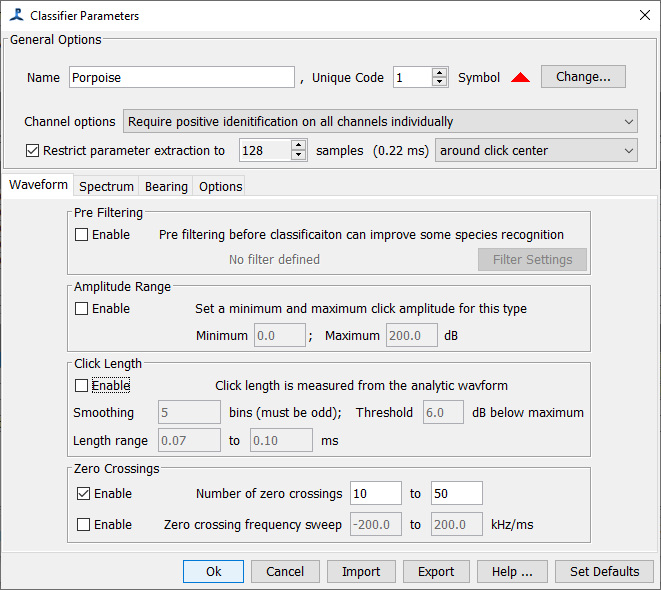
\includegraphics[keepaspectratio]{images/reclass2.png}}

}

\subcaption{\label{fig-reclass2}Setup for a Porpoise click classifier}

\end{minipage}%

\caption{\label{fig-reclass}Configuring click classifiers prior to
running reclassification}

\end{figure}%

\subsection{Run the task on all five
datasets}\label{run-the-task-on-all-five-datasets}

If you're using the batch processor configuration that you used to
process the raw data, then it will still be saying that all jobs are
complete. To reset them ready for running the offline tasks, right click
anywhere in the jobs table and select \emph{Reprocess all jobs} from the
dropdown menu.

Make sure that you've selected the appropriate checkbox to run the
Reclassification offline task.

Then, just as before, press the red start button. Each dataset will open
in turn and the selected offline task will run on each dataset,
following the same rules as earlier as to how many jobs will run
concurrently.

Running the click classification is a lot quicker than processing the
raw data, so this should only take a couple of minutes to run on most
computers. Once jobs are complete, you can view the data for each job
using the
\href{https://www.pamguard.org/olhelp/overview/PamMasterHelp/docs/viewerMode.html}{PAMGuard
viewer}.

\section{Acknowledgements}\label{acknowledgements}

Funding for the development of the Batch Processing module was provided
by the Bureau of Oceans Management (BOEM), Contract number
140M0122C0006.




\end{document}
